\documentclass[12pt,a4paper]{article}
\usepackage[utf8]{inputenc}
\usepackage{amsmath}
\usepackage{amsfonts}
\usepackage{amssymb}
\usepackage{graphicx}
\usepackage[spanish]{babel} 
\usepackage[fixlanguage]{babelbib}
\usepackage[none]{hyphenat}
\usepackage[hidelinks]{hyperref}
\usepackage{titlesec}
\usepackage{titling} 
\usepackage{smartdiagram}
\usepackage{multicol} 
\usepackage{appendix}
\usepackage{tikz}
%\usepackage{subfig}
\usepackage{alltt}
\usepackage{spverbatim}
\usepackage{subfigure}
\usetikzlibrary{positioning}
\usepackage{listings,xcolor}
\usetikzlibrary {positioning}
\definecolor {processblue}{cmyk}{0.96,0,0,0}
\selectbiblanguage{spanish}

%\setlist[itemize]{noitemsep}
%\usetikzlibrary{shapes.symbols}
%\usepackage[hmarginratio=1:1,top=32mm,columnsep=20pt]{geometry}
\setlength{\parskip}{2mm}
%\tikzset{description title/.append style={
%		signal, 
%		signal to=south, 
%		signal from=north,
%		yshift=-0.65cm,
%	}
%}
\lstset{
	string=[s]{"}{"},
	stringstyle=\color{blue},
	comment=[l]{:},
	commentstyle=\color{black},
}


\makeatletter
\newenvironment{code}
{\RecustomVerbatimEnvironment{Verbatim}{BVerbatim}{}%
	\def\FV@BProcessLine##1{%
		\hbox{%
			\hbox to\z@{\hss\kern\FV@NumberSep}%
			\FancyVerbFormatLine{##1}%
		}%
	}%
	\VerbatimEnvironment
	\setbox\z@=\hbox\bgroup
	\begin{minted}{js}}
	{\end{minted}\egroup
	\leavevmode\vbox{\hrule\kern2mm\box\z@\kern2mm\hrule}}
\makeatother

\title{PEC 2}


\setlength{\droptitle}{-5\baselineskip} % Move the title up
\pretitle{\begin{center}\Huge\bfseries} % Article title formatting
	\posttitle{\end{center} \vspace{-15pt}} % Article title closing formatting



\title{Práctica II\\Tipología \\ y \\Ciclo de Vida de los datos \\} % Article title
\author{%
		\protect
\includegraphics[trim = 0mm 0mm 0mm 0mm, clip,scale=0.3]{images/uoc}\\ %53 en 3 quito titulo
	\textsc{Gregorio Andrés García Menéndez} \\ % Your name
	\textsc{ Manuel Gómez Montero}
		%\normalsize \href{mailto:mnlgmontero@uoc.edu}{mnlgmontero@uoc.edu}  
% Your email address
	%\and % Uncomment if 2 authors are required, duplicate these 4 lines if more
	%\textsc{Jane Smith}\thanks{Corresponding author} \\[1ex] % Second author's name
	%\normalsize University of Utah \\ % Second author's institution
	%\normalsize \href{mailto:jane@smith.com}{jane@smit\clearpageh.com} % Second author's email address
}
\date{\today} % Leave empty to omit a date
%\renewcommand{\maketitlehookd}{%

\makeindex
\begin{document}
	\nocite{*}
	\maketitle
\tableofcontents
\clearpage

\section{Introducción}

\subsection{Objetivos}
Los objetivos de esta práctica son:
\begin{itemize}
\item Aprender a aplicar los conocimientos adquiridos y su capacidad de resolución de problemas en entornos nuevos o poco conocidos dentro de contextos más amplios o multidisciplinares.
\item Saber identificar los datos relevantes y los tratamientos necesarios (integración, limpieza y validación) para llevar a cabo un proyecto analítico.
\item Aprender a analizar los datos adecuadamente para abordar la información contenida en los datos.
\item Identificar la mejor representación de los resultados para aportar conclusiones sobre el problema planteado en el proceso analítico.
\item Actuar con los principios éticos y legales relacionados con la manipulación de datos en función del ámbito de aplicación.
\item Desarrollar las habilidades de aprendizaje que les permitan continuar estudiando de un modo que tendrá que ser en gran medida autodirigido o autónomo.
\item Desarrollar la capacidad de búsqueda, gestión y uso de información y recursos en el ámbito de la ciencia de datos.
\end{itemize}


\subsection{Descripción del Dataset}
El dataset escogido ha sido obtenido a través de una encuesta de estudiantes de secundaria que asisten a cursos de matemáticas y  portugués. Este conjunto de datos contiene bastante información de interés sobre los estudiantes. Aunque incialmente el objetivo principal del dataset era ver el consumo de alcohol en estudiantes según variables sociodemográficas, dicho dataset contiene suficiente información para otro tipo de estudios, centrados por ejemplo en la calificación de los alumnos.

Los datos han sido obtenidos de \textit{Kaggle} y se encuentran en dos ficheros \textit{CSV} independientes, uno para la asignatura de matemáticas y otro para la de portugués. Cada uno de estos ficheros contiene las siguientes variables: 

\begin{enumerate}
	\item \textit{school}: Define la escuela del estudiante. Puede ser ``GP'' (Gabriel Pereira) o ``MS'' (Mousinho da Silveira).
	\item \textit{sex}: Indica el sexo del estudiante.
	\item \textit{age}: Se refiere a la edad del estudiante.
	\item \textit{address}: Indica si el estudiante vive en zona urbana o rural.
	\item \textit{famsize}: Define si la familia se compone de menos de tres miembros o de tres o más.
	\item \textit{Pstatus}: Se refiere al estado de los padres, si viven juntos o no.
	\item \textit{Medu}: Nivel de educación de la madre (0: Ninguna, 1: Primaria (hasta 4º), 2: Primaria (Desde 5º), 3: Secundaria o  4: Educación superior).
	\item \textit{Fedu}: Nivel de educación del padre (0: Ninguna, 1: Primaria (hasta 4º), 2: Primaria (Desde 5º), 3: Secundaria o  4: Educación superior).
	\item \textit{Mjob}:  Trabajo de la madre.
	\item \textit{Fjob}: Trabajo del padre.
	\item \textit{reason}: Razón por la que se escoge esta escuela.
	\item \textit{guardian}: Tutor del alumno.
	\item \textit{traveltime}: Tiempo de camino a la escuela  (1: <15 min., 2: 15 to 30 min., 3: 30 min. a 1 hora,4: >1 hora).
	\item \textit{studytime}: Tiempo de estudio semanal ( 1: <2 horas, 2: 2 a 5 horas, 3: 5 a 10 horas o  4: >10 horas).
	\item \textit{failures} - Número de fracasos en clases pasadas (4 para 4 o más)
	\item \textit{schoolsup} - Define si el estudiante recibe o no clases particulares. 
	\item \textit{famsup} - Indica si el estudiante recibe apoyo educativo familiar.
	\item \textit{paid}: Clases extra pagadas dentro de la asignatura del curso. 
	\item \textit{activities}: Actividades extraescolares.
	\item \textit{nursery}: Indica si asistió a la guardería. 
	\item \textit{higher}: Define si el estudiante tiene intención de  realizar estudios superiores.
	\item \textit{internet}: Indica si el estudiante posee internet en casa.
	\item \textit{romantic}: Define si el estudiante tiene una relación amorosa. 
	\item \textit{famrel}: Calidad de las relaciones familiares (De 1 a 5 de peor a mejor).
	\item \textit{freetime}: Indica la cantidad de tiempo libre del estudiante (De 1 a 5 de menos a más).
	\item \textit{goout}: Mide la frecuencia con la que el estudiante sale con amigos (De 1 a 5 de menos a más).
	\item \textit{Dalc} -Consumo de alcohol entre semana (De 1 a 5 de menos a más).
	\item \textit{Walc} - Consumo de alcohol los fines de semana (De 1 a 5 de menos a más).
	\item \textit{health} - Mide el estado de salud del estudiante (De 1 a 5 de peor a mejor).
	\item \textit{absences}: Número de ausencias a clase.
	\item \textit{G1}: Calificación del primer periodo.
	\item \textit{G2}: Calificación del segundo periodo.
	\item \textit{G3}: Calificación final.
\end{enumerate}




\section{Limpieza de datos}
\subsection{Unión de conjuntos}
El primer paso consiste en unir ambos conjuntos de datos de cada clase para tener un único dataset que será el que utilizaremos en el resto del documento.

Según se indica en Kaggle existen 382 estudiantes que asisten a ambos cursos. Como cada alumno en los dos ficheros no viene identificado con un \textit{id} único, explican que estos estudiantes pueden ser identificados por el mismo valor de las siguientes características en ambos ficheros: colegio, sexo, edad, dirección, tamaño de familia, trabajo y nivel de educación de los padres, razón por la que ha elegido el colegio, si han asistido a la guardería y si poseen internet en casa. 

Sin embargo creemos que además de estas características hay otras que no pueden variar en un mismo estudiante en ambos ficheros como son: el tiempo de camino a la escuela, número de fracasos en clases pasadas, si realiza actividades extraescolares, si tiene intención de realizar estudios superiores, si tiene una relación, la calidad de las relaciones, la frecuencia de salidas con amigos, la cantidad consumida de alcohol y el estado de salud. Con esta separación vemos que existen 320 estudiantes que asisten a ambas clases. 

Comparando los valores de ambos cursos del resto del variables vemos que también coinciden en ambos cursos el tutor del alumno, si recibe soporte familiar y el tiempo de estudio. 


 \begin{figure}[ht!]
	\centering
	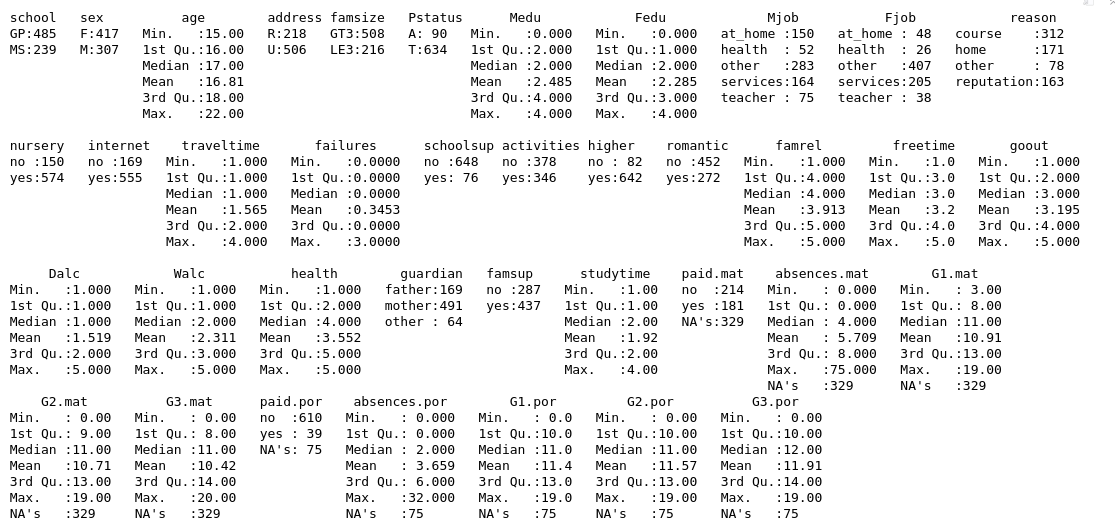
\includegraphics[trim = 0mm 0mm 0mm 0mm, clip,scale=0.4]{images/summary_inicial}
	\caption{Summary dataset conjunto}
	\label{fig:sum1}
\end{figure}


El dataset resultado de la unión posee un total de 724 alumnos 75 de los cuales solo asisten a matemáticas, 329 solo a portugués y  320 a ambos cursos.


\subsection{Tratamiento de NAs}
En primer lugar vamos a encargarnos de los valores perdidos que se dan unicamente en los casos de que los alumnos no hayan asistido a alguno de los cursos, una opción sería eliminar los datos de cualquier alumno que no posea datos en algunos de los cursos, pero implicaría quedarnos solo con un 44\% de los datos. 


Por lo tanto la opción escogida para los valores perdidos es la siguiente: 


 \begin{figure}[ht!]
	\centering
	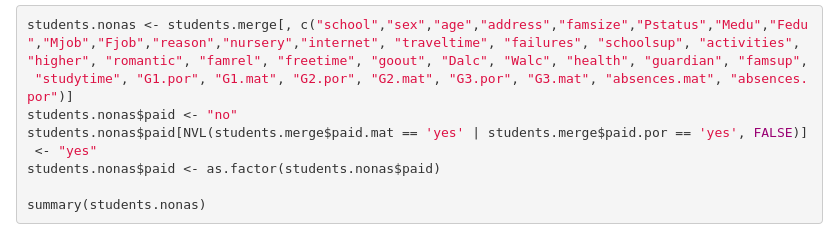
\includegraphics[trim = 0mm 0mm 0mm 0mm, clip,scale=0.5]{images/nonas_paid}
	\caption{Unificación variable paid}
	\label{fig:nonas_paid}
\end{figure}


\begin{itemize}
	\item \textit{paid}: Unificaremos las variables de ambos cursos tomando un valor ``yes'' cuando el alumno de clases extras pagadas de alguno de los cursos.
	\item \textit{calificaciones} y {absences}: Utilizaremos el método \textit{missForest} que utiliza árboles de decisión para imputar los valores perdidos en variables tanto numéricas como categóricas.  
	 
\end{itemize}

 \begin{figure}[ht!]
	\centering
	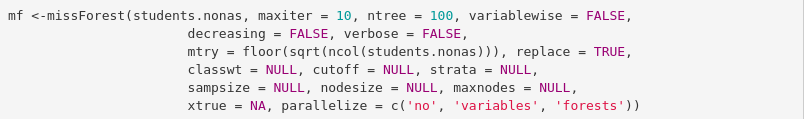
\includegraphics[trim = 0mm 0mm 0mm 0mm, clip,scale=0.5]{images/nonas_cal}
	\caption{Imputación valores perdidos con missForest}
	\label{fig:nonas_cal}
\end{figure}



 \begin{figure}[ht!]
	\centering
	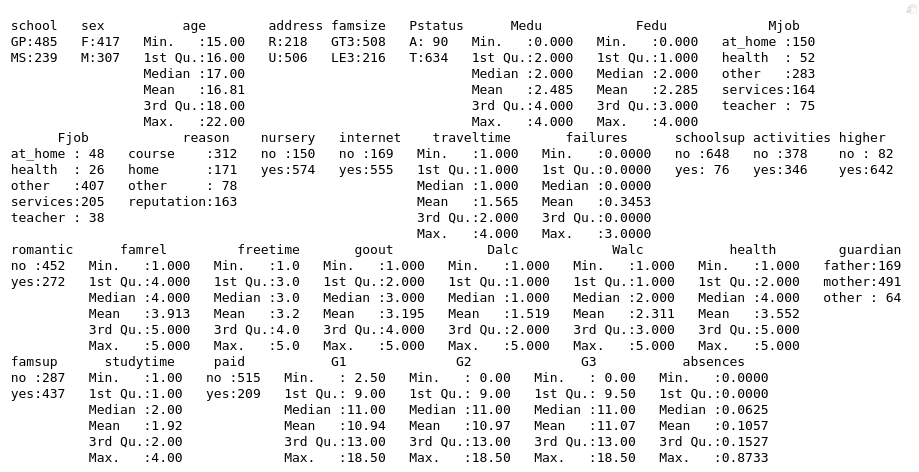
\includegraphics[trim = 0mm 0mm 0mm 0mm, clip,scale=0.4]{images/summary_nonas}
	\caption{Summary dataset sin NAs}
	\label{fig:sum2}
\end{figure}



En el notebook se pueden ver los detalles de estos procesos en la figura \ref{fig:sum2} podemos ver la salida del comando \textit{summary} para este nuevo dataset.


\subsection{Análisis de 0s}
Vamos a analizar uno por uno los casos en los que existen valores 0 y a definir si son valores posibles de la variable o por el contrario se trata de valores vacíos indicados como 0. Las variables que contienen valores 0 son:


 \begin{figure}[ht!]
	\centering
	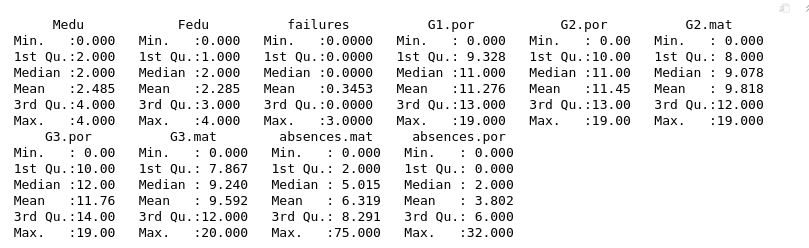
\includegraphics[trim = 0mm 0mm 0mm 0mm, clip,scale=0.4]{images/summary_0s}
	\caption{Summary atributos con 0s}
	\label{fig:sum_0s}
\end{figure}


Para el caso de la educación del padre y la madre ya definimos que el valor 0 significa que no poseen ningún tipo de educación.

Para el resto de casos vemos que el valor 0 también es posible ya que:

\begin{itemize}
	 

\item Es posible no haber suspendido ninguna asignatura, de hecho más del 75\% de alumnos así lo han hecho.
\item En las calificaciones es posible sacar un 0.
\item En el caso de las ausencias también existen alumnos que no han faltado a ninguna clase. En el caso \item de las clases de portugués más del 25\%.
\end{itemize}


\subsection{Selección de variables/Reducción de dimensionalidad}
Observando el dataset vemos que, aún tras la unión de los datasets, tenemos una gran cantidad de dimensiones, en concreto 37, lo que puede dificultar nuestro análisis. En esta primera fase vamos a hacer una primera aproximación para reducir la dimensionalidad. Posteriormente en los primeros apartados del análisis estadístico reduciremos aún más esta dimensionalidad.

En primer lugar existen variables que, a priori, tienen poca significancia para nuestro análisis como puede ser la escuela a la que asiste el alumno, por lo que podemos eliminar esta variable. 

Por otro lado podemos agrupar las calificaciones en una única variable que nos indique la calificación media del alumno. 


\begin{figure}[ht!]
	\centering
	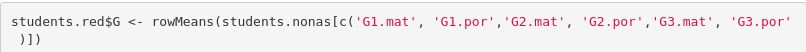
\includegraphics[trim = 0mm 0mm 0mm 0mm, clip,scale=0.5]{images/red_calif}
	\caption{Unificación calificaciones}
	\label{fig:redcal}
\end{figure}


También vamos a realizar el mismo paso para las audiencia, pero observando los datos parece que las ausencias son mayores en matemáticas. Como lo que nos interesa es saber los alumnos que han faltado más o menos veces y queremos evitar que tenga un mayor peso los alumnos de matemáticas, normalizaremos estos valores antes de realizar la media. 

\begin{figure}[ht!]
	\centering
	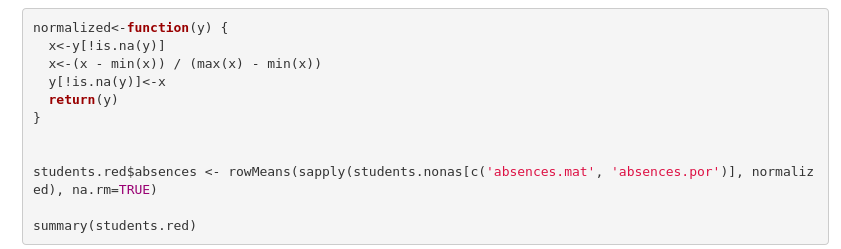
\includegraphics[trim = 0mm 0mm 0mm 0mm, clip,scale=0.5]{images/red_aus}
	\caption{Unificación ausencias}
	\label{fig:redaus}
\end{figure}



Con estos detalles que pueden observarse en el notebook vemos que hemos conseguido reducir a 30 la dimensionalidad con las variables que aparecen en la figura \ref{fig:sum_red}.


\begin{figure}[ht!]
\centering
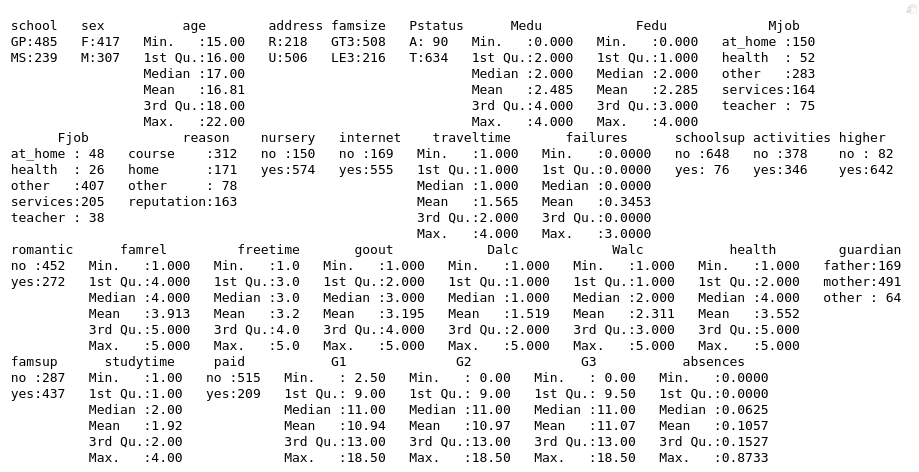
\includegraphics[trim = 0mm 0mm 0mm 0mm, clip,scale=0.4]{images/summary_nonas}
\caption{Summary dataset reducido}
\label{fig:sum_red}
\end{figure}


\subsection{Tipos de Variables}
En los tipos mostrados hay algunos que no es correcto el tipo. En la educación tanto de la madre como del padre consideramos que aunque se use un número para la representación debería ser un factor. Lo mismo ocurre para el tiempo de viaje o el tiempo de estudio.  Podemos encontrar más detalles en el notebook. 


La explicación de considerar el tiempo de estudio y el tiempo de viaje es que, aunque pueden parecer numéricas, en realizar son factores. En la descripción del dataset aparece explicado:

studytime: Weekly study time: (numeric: 1 - $<$2 hours, 2 - 2 to 5 hours, 3 - 5 to 10 hours, or 4 - $>$10 hours)
traveltime: Home to school travel time (numeric: 1 - $<$15 min., 2 - 15 to 30 min., 3 - 30 min. to 1 hour, or 4 - $>$1 hour)

Por lo tanto, al ser categorías, las tratamos como factores y no como numéricas.


\subsection{Análisis de Outliers}
Para las variables numéricas realizamos un estudio de outliers. En nuestro caso, las variables a estudiar son ``age'' y ``G''. El resto de variables numéricas en realidad no lo son, puesto que son categóricas. Por ejemplo: "studytime" va de 1 a 4, y no hace referencia a las horas que el alumno pasa estudiando, sino que son categorías equivalentes a por ejemplo: Nada, Poco, Normal, Mucho. Podría haber valores erróneos debido a la transcripción de los datos o similar, pero dichos errores ya los hubiéramos detectado en la creación del data set, ya que gracias a la función ``summary'' vemos los valores mínimos y máximos y para estas variables categóricas numéricas no hay valores erróneos (mínimo y máximo corresponden a las categorías mínimas y máximas).

Procedemos al estudio de age y G:

\begin{figure}[h]
  \centering
  \begin{minipage}[b]{0.4\textwidth}
    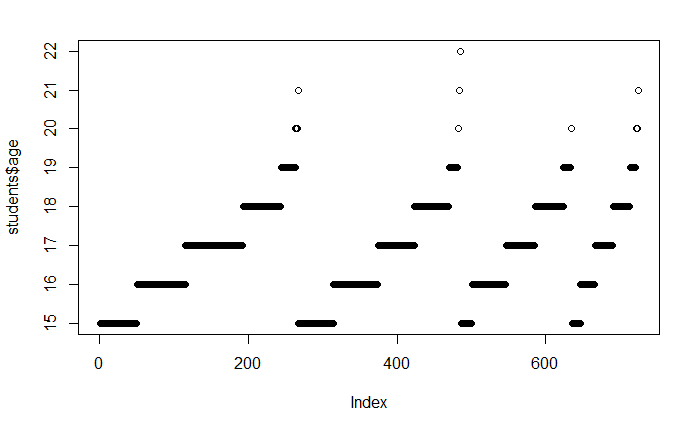
\includegraphics[trim = 0mm 0mm 0mm 0mm, clip,scale=0.4]{images/outliers_age_1}
    \caption{Distribución de la variable Age}
  \end{minipage}
  \hfill
  \begin{minipage}[b]{0.4\textwidth}
    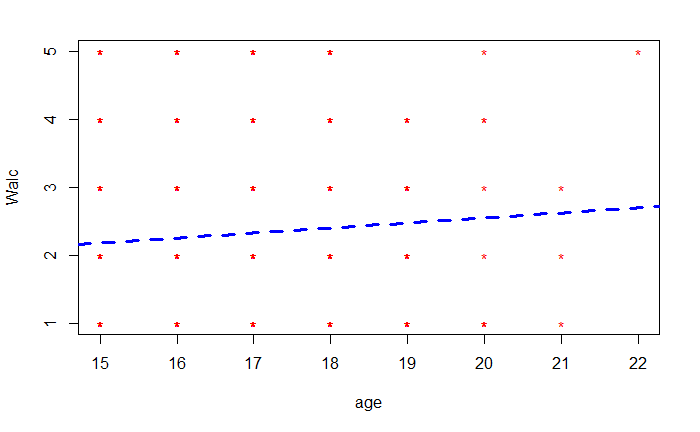
\includegraphics[trim = 0mm 0mm 0mm 0mm, clip,scale=0.4]{images/outliers_age_2}
    \caption{Walc en función de Age con outliers. Modelo lineal en azul.}
  \end{minipage}
  \hfill  
  \begin{minipage}[b]{0.4\textwidth}
    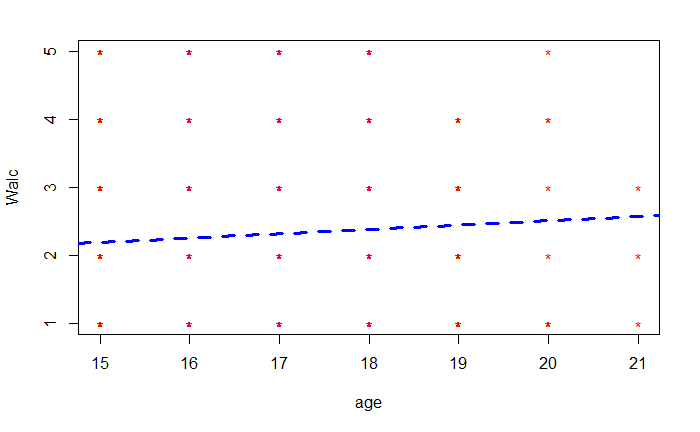
\includegraphics[trim = 0mm 0mm 0mm 0mm, clip,scale=0.4]{images/outliers_age_3}
    \caption{Walc en función de Age sin outliers. Modelo lineal en azul.}
  \end{minipage}
\end{figure}


Como podemos ver, para el campo edad los alumnos van de los 15 a los 22, siendo las franjas más pobladas los 15, 16 y 17 años. Al haber valores intermedios que en número van disminuyendo gradualmente desde los 18 hasta los 22, no consideramos ningún valor extremo (como el único estudiantes de 22 años) como valor erróneo. Además, al ser tan pocos estudiantes, no los descartamos en nuestros estudios ya que pueden aportar información valiosa, y como podemos ver en la comparativa del conjunto con outliers y sin outliers, no cambia de forma crítica.

\begin{figure}[h]
  \centering
  \begin{minipage}[b]{0.4\textwidth}
    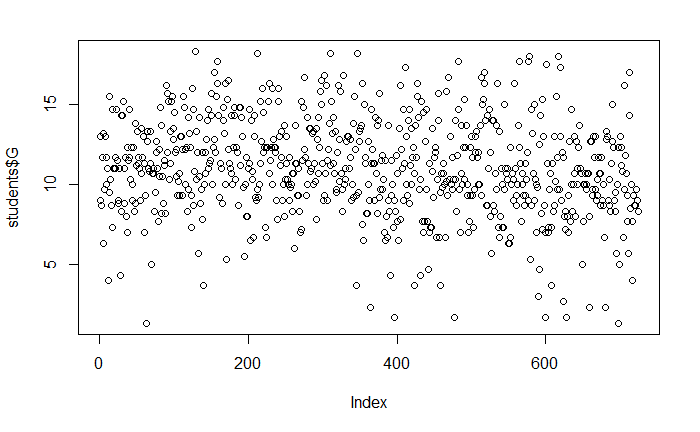
\includegraphics[trim = 0mm 0mm 0mm 0mm, clip,scale=0.4]{images/outliers_g_1}
    \caption{Distribución de la variable G}
  \end{minipage}
  \hfill
  \begin{minipage}[b]{0.4\textwidth}
    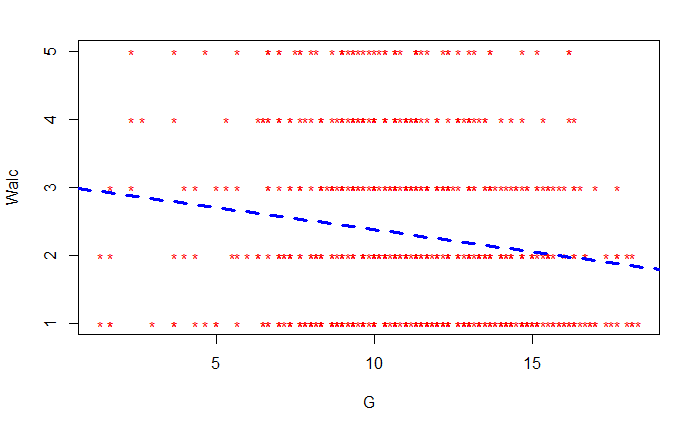
\includegraphics[trim = 0mm 0mm 0mm 0mm, clip,scale=0.4]{images/outliers_g_2}
    \caption{Walc en función de G. Modelo lineal en azul.}
  \end{minipage}
\end{figure}

En el caso de la media de la nota G es más claro todavía. Los datos no demuestran valores extremos que se puedan deber a errores, y aquellos más alejados de la mayor concentración de estudiantes son valores que aportan información para los estudios que vamos a realizar en cuanto al consumo de alcohol y de desempeño estudiantil.


\section{Análisis Estadístico}
\subsection{Análisis gráfico inicial}
Observando las gráficas vemos que hay variables que parece que sí tienen influencia a simple vista en el consumo de alcohol tanto a diario como los fines de semana, como pueden ser el sexo y el estado de los padres. Sin embargo vemos otros que, a priori, no parece que tengan influencia así que en un primer momento vamos a dejar fuera del análisis la dirección, si el alumno tiene internet, si tiene una relación, el tutor, si realiza actividades extraescolares o si recibe clases de pago. 


En este apartado vamos a mostrar únicamente las gráficas de las variables que hemos descartado en el estudio inicial, para ver que, efectivamente, a priori no tienen influencia en el consumo de alcohol. Las gráficas completas se muestran en el \textit{notebook}. 


\begin{figure}[ht!]
	\subfigure[Fin de semana]{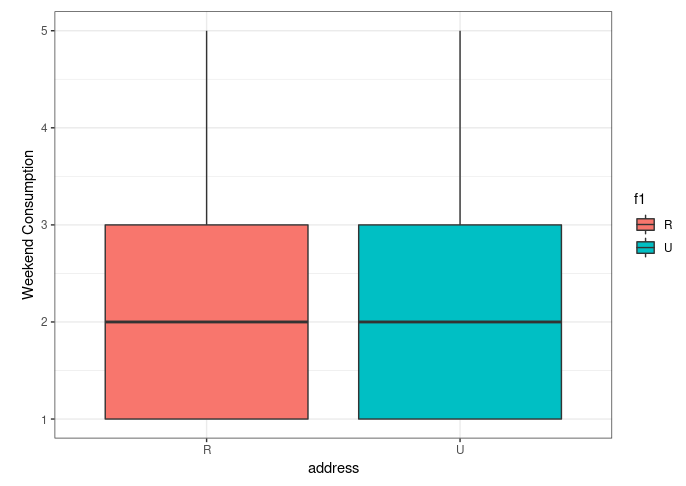
\includegraphics[trim = 0mm 0mm 20mm 0mm, clip,scale=0.27]{images/bp_address_weekend.png}}\hfill
	\subfigure[Diario]{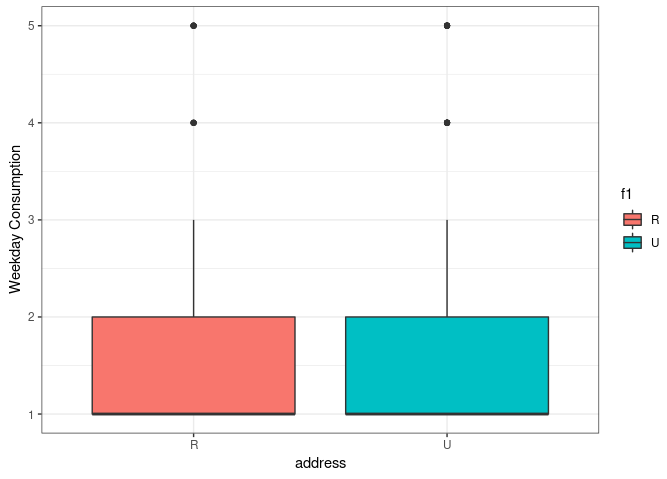
\includegraphics[trim = 0mm 0mm 20mm 0mm, clip,scale=0.27]{images/bp_address_week.png}}
	 \caption{Boxplot dirección - consumo alcohol}
	 \label{fig:bpaddress}
\end{figure}

 \begin{figure}[hbp!]
 	\subfigure[Fin de semana]{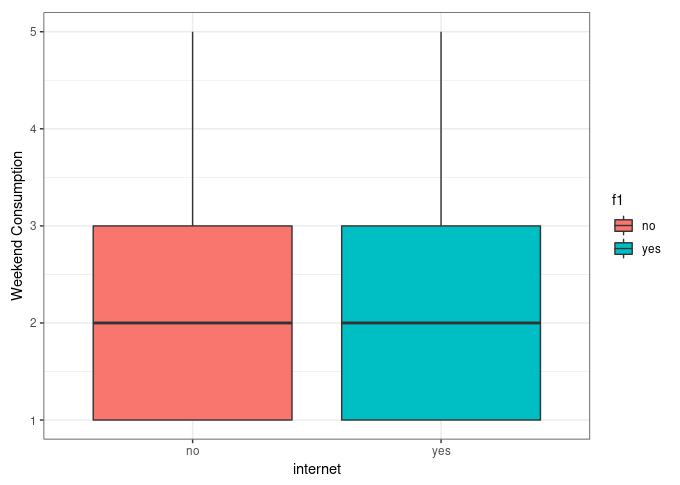
\includegraphics[trim = 0mm 0mm 23mm 0mm, clip,scale=0.27]{images/bp_inet_weekend.png}}\hfill
 	\subfigure[Diario]{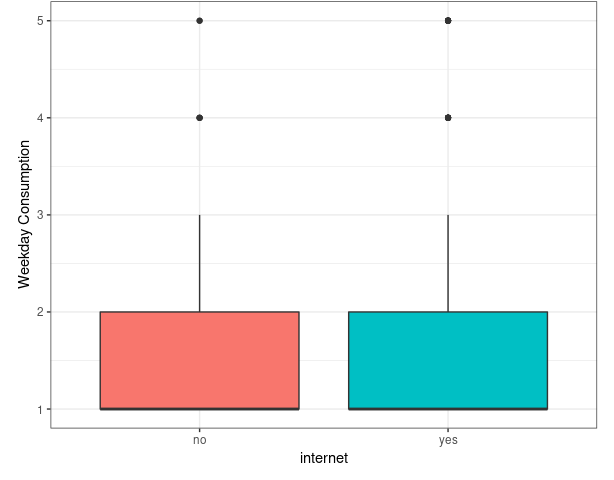
\includegraphics[trim = 0mm 0mm 0mm 0mm, clip,scale=0.27]{images/bp_inet_week.png}}
 	\caption{Boxplot Internet - consumo alcohol}
 	\label{fig:bpinet}
 \end{figure}


\begin{figure}[ht!]
	\subfigure[Fin de semana]{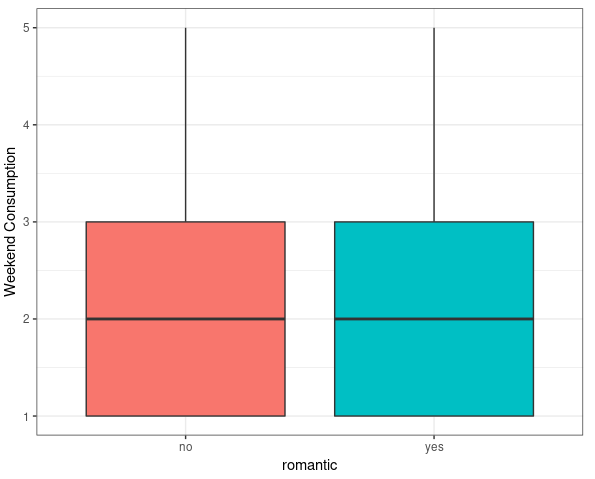
\includegraphics[trim = 0mm 0mm 0mm 0mm, clip,scale=0.27]{images/bp_rom_weekend.png}}\hfill
	\subfigure[Diario]{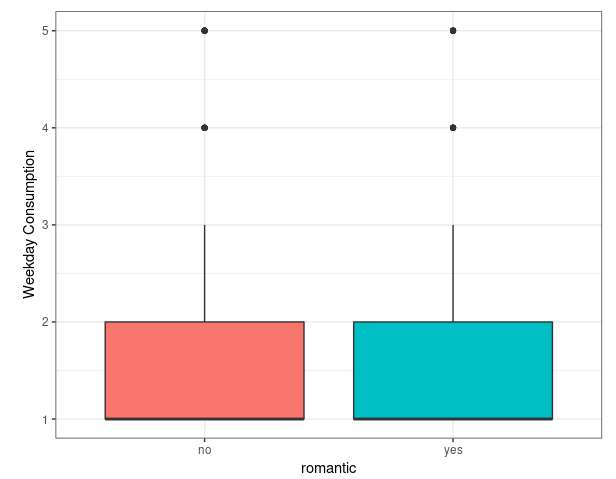
\includegraphics[trim = 0mm 0mm 0mm 0mm, clip,scale=0.27]{images/bp_rom_week.png}}
	\caption{Boxplot relación romántica - consumo alcohol}
	\label{fig:bprom}
\end{figure}


\begin{figure}[ht!]
	\subfigure[Fin de semana]{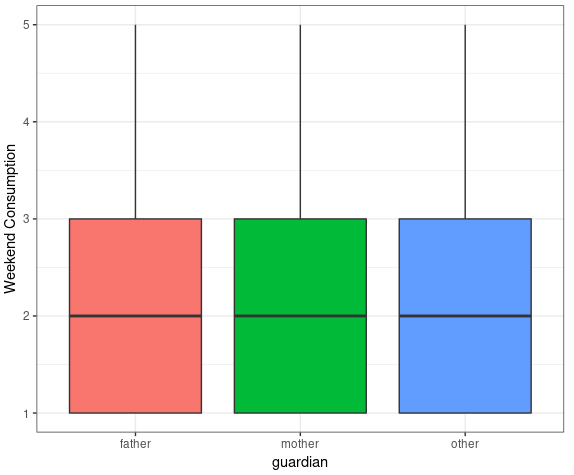
\includegraphics[trim = 0mm 0mm 0mm 0mm, clip,scale=0.27]{images/bp_tutor_weekend.png}}\hfill
	\subfigure[Diario]{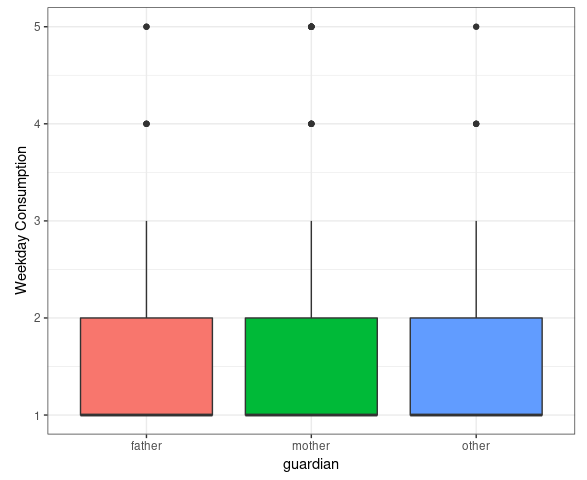
\includegraphics[trim = 0mm 0mm 0mm 0mm, clip,scale=0.27]{images/bp_tutor_week.png}}
	\caption{Boxplot tutor - consumo alcohol}
	\label{fig:bptutor}
\end{figure}



\begin{figure}[ht!]
	\subfigure[Fin de semana]{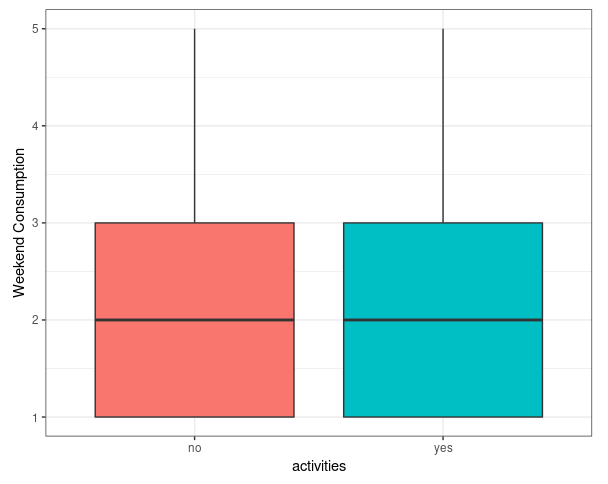
\includegraphics[trim = 0mm 0mm 0mm 0mm, clip,scale=0.27]{images/bp_act_weekend.png}}\hfill
	\subfigure[Diario]{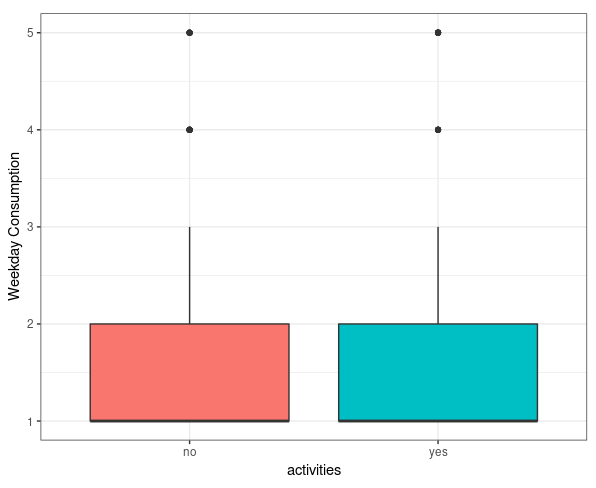
\includegraphics[trim = 0mm 0mm 0mm 0mm, clip,scale=0.27]{images/bp_act_week.png}}
	\caption{Boxplot actividades extraescolares - consumo alcohol}
	\label{fig:bpact}
\end{figure}



\begin{figure}[ht!]
	\subfigure[Fin de semana]{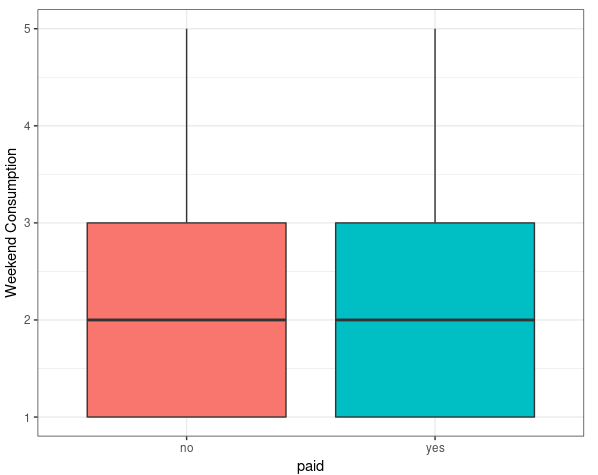
\includegraphics[trim = 0mm 0mm 0mm 0mm, clip,scale=0.27]{images/bp_paid_weekend.png}}\hfill
	\subfigure[Diario]{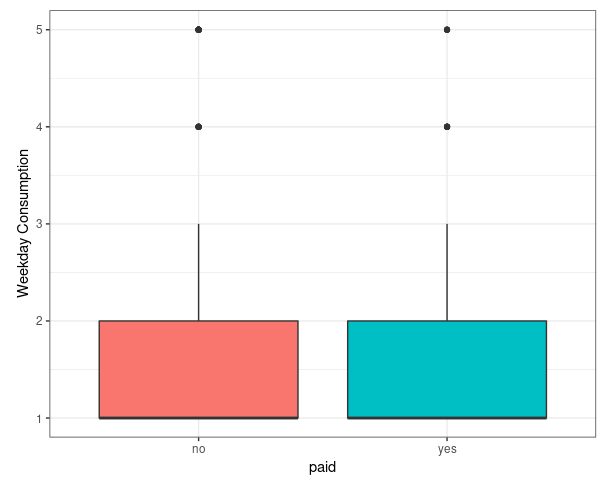
\includegraphics[trim = 0mm 0mm 0mm 0mm, clip,scale=0.27]{images/bp_paid_week.png}}
	\caption{Boxplot clases pago - consumo alcohol}
	\label{fig:bppaid}
\end{figure}


\begin{figure}[ht!]
	\centering
	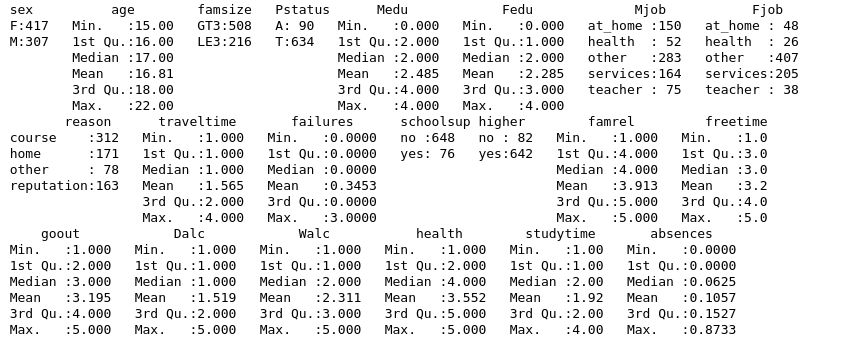
\includegraphics[trim = 0mm 0mm 0mm 0mm, clip,scale=0.4]{images/summary_final}
	\caption{Summary dataset final}
	\label{fig:sum4}
\end{figure}







En la figura \ref{fig:sum4} podemos ver el resumen del dataset. Tras la fase de limpieza y este pequeño análisis hemos pasado de tener dos datasets con 33 dimensiones a \textbf{un único dataset con 21 dimensiones} pasando por un dataset conjunto de 41 dimensiones.  


\clearpage

\subsection{ Estadística Inferencial}
En este apartado vamos a ver si hay diferencia significativas en el consumo de alcohol a diario y fines de semana entre estudiantes en función del sexo y de situación de los padres. También veremos si el consumo de alcohol es distinto entre estudiantes que aprueban y que suspenden:
  
Se trata de un problema de diferencia de medias entre dos muestras en el que no conocemos la varianza poblacional. Tampoco sabemos a priori si los datos siguen una distribución normal, pero el tamaño de las muestras es lo suficientemente grande para tener en cuenta el teorema del límite central.


Para cada caso la hipótesis sería: 

$$
\left\{
\begin{array}{ll}
H_{0}: &  \mu_{g1}-\mu_{g2}=0\\
H_{1}: & \mu_{g1}-\mu_{g2}\ne0
\end{array}
\right.
$$


\subsubsection{Estudiantes de distinto sexo}

Separamos el consumo de alcohol los fines de semana en dos conjunto según el sexo:

\begin{spverbatim}
data_weekend_sex_m <- students$Walc[students$sex == 'M'] 
data_weekend_sex_f <- students$Walc[students$sex == 'F'] 

t.test(data_weekend_sex_m, data_weekend_sex_f, var.equal = TRUE, conf.level = 0.95)

Two Sample t-test

data:  data_weekend_sex_m and data_weekend_sex_f
t = 9.7324, df = 722, p-value < 2.2e-16
alternative hypothesis: true difference in means is not equal to 0
95 percent confidence interval:
 0.7114636 1.0710375
sample estimates:
mean of x mean of y 
 2.824104  1.932854
\end{spverbatim}

Por el p-value vemos que no podemos aceptar la hipótesis nula, y concluimos que al 95\% de nivel de confianza los estudiantes masculinos y femeninos no tienen el mismo consumo de alcohol los fines de semana. 


Realizamos las mismas operaciones para el consumo de alcohol entre semana:

\begin{spverbatim}
data_weekday_sex_m <- students$Dalc[students$sex == 'M'] 
data_weekday_sex_f <- students$Dalc[students$sex == 'F'] 

t.test(data_weekday_sex_m, data_weekday_sex_f, var.equal = TRUE, conf.level = 0.95)

Two Sample t-test

data:  data_weekday_sex_m and data_weekday_sex_f
t = 8.2948, df = 722, p-value = 5.321e-16
alternative hypothesis: true difference in means is not equal to 0
95 percent confidence interval:
 0.4211673 0.6823564
sample estimates:
mean of x mean of y 
 1.837134  1.285372

\end{spverbatim}

Por el p-value vemos que ocurre lo mismo que en los fines de semana. No podemos acepta la hipotésis nula y al 95\% afirmamos que hay diferencia en el consumo de alcohol entre estudiantes masculinos y femeninos para los días entre semana.


\subsubsection{Estudiantes con diferente situación de convivencia de los padres}

Ahora realizamos el estudio para el consumo de alcohol según la situación de los padres de cada alumno:

Primero, en fines de semana:
\begin{spverbatim}
data_weekend_pstatus_t <- students$Walc[students$Pstatus == 'T'] 
data_weekend_pstatus_a <- students$Walc[students$Pstatus == 'A'] 

t.test(data_weekend_pstatus_t, data_weekend_pstatus_a, var.equal = TRUE, conf.level = 0.95)

Two Sample t-test

data:  data_weekend_pstatus_t and data_weekend_pstatus_a
t = 1.3035, df = 722, p-value = 0.1928
alternative hypothesis: true difference in means is not equal to 0
95 percent confidence interval:
 -0.09613914  0.47601996
sample estimates:
mean of x mean of y 
 2.334385  2.144444

\end{spverbatim}
En el caso del consumo en los fines de semana, no hay diferencias significativas en función del estado de convivencia de los padres a un 95\% de nivel de confianza.


Ahora, para el consumo entre semana:
\begin{spverbatim}
data_weekday_pstatus_t <- students$Dalc[students$Pstatus == 'T'] 
data_weekday_pstatus_a <- students$Dalc[students$Pstatus == 'A'] 

t.test(data_weekday_pstatus_t, data_weekday_pstatus_a, var.equal = TRUE, conf.level = 0.95)

Two Sample t-test

data:  data_weekday_pstatus_t and data_weekday_pstatus_a
t = 0.69872, df = 722, p-value = 0.4849
alternative hypothesis: true difference in means is not equal to 0
95 percent confidence interval:
 -0.1318160  0.2774872
sample estimates:
mean of x mean of y 
 1.528391  1.455556

\end{spverbatim}
Con un p-value tan alto aceptamos la hipótesis nula, concluyendo que el consumo de alcohol entre semana es el mismo para estudiantes cuyos padres viven juntos y para estudiatnes cuyos padres viven separados.


\subsubsection{Estudiantes que aprueban ($G >= 10$) y estudiantes que suspenden ($G < 10$)}
  
Por último, realizamos el estudio para el consumo de alcohol según las calificaciones que obtiene el alumno (si aprueba o suspende):

En el caso del consumo los fines de semana:
\begin{spverbatim}
data_weekend_aprobados <- students$Walc[students$G >= 10] 
data_weekend_suspensos <- students$Walc[students$G < 10] 

t.test(data_weekend_aprobados, data_weekend_suspensos, var.equal = TRUE, conf.level = 0.95)

Two Sample t-test

data:  data_weekend_aprobados and data_weekend_suspensos
t = -2.8183, df = 722, p-value = 0.00496
alternative hypothesis: true difference in means is not equal to 0
95 percent confidence interval:
 -0.4842420 -0.0865913
sample estimates:
mean of x mean of y 
 2.214583  2.500000
 
\end{spverbatim}
Con un p-value menor que 0.05, al 95\% de confianza afirmamos que sí hay diferencia en el consumo de alcohol los fines de semana en función de si el alumno aprueba o no.

\begin{spverbatim}
data_weekday_aprobados <- students$Dalc[students$G >= 10] 
data_weekday_suspensos <- students$Dalc[students$G < 10] 

t.test(data_weekday_aprobados, data_weekday_suspensos, var.equal = TRUE, conf.level = 0.95)

Two Sample t-test

data:  data_weekday_aprobados and data_weekday_suspensos
t = -2.7561, df = 722, p-value = 0.005996
alternative hypothesis: true difference in means is not equal to 0
95 percent confidence interval:
 -0.34170360 -0.05740842
sample estimates:
mean of x mean of y 
 1.452083  1.651639 
 
\end{spverbatim}
Viendo el p-value, podemos decir al 95% que también hay diferencias entre alumnos que aprueban y alumnos que suspenden en cuanto al consumo de alcohol entre semana.

\subsection{Modelo de regresión lineal}

En este apartado aplicaremos un modelo de regresión lineal múltiple que use como variables explicativas cuánto sale el estudiante con amigos, cuánto bebe entre semana, su sexo y su edad.

Al usar regresores cualitativos, es importante definir una categoría de referencia, para lo que usaremos la función de R *relevel* estableciendo la categoría "F" como referente para el sexo. El resultado lo almacenamos en una nueva variable.

\begin{spverbatim}
students$sexR <- relevel(students$sex, "F")
modelo <- lm(Walc ~ goout + sexR + Dalc + age + studytime, data = students )
summary(modelo)

Call:
lm(formula = Walc ~ G + sexR + Dalc + studytime + goout, data = students)

Residuals:
    Min      1Q  Median      3Q     Max 
-3.3617 -0.6975 -0.1785  0.6505  2.8745 

Coefficients:
            Estimate Std. Error t value Pr(>|t|)    
(Intercept)  0.42554    0.18484   2.302   0.0216 *  
G           -0.01084    0.01189  -0.912   0.3623    
sexRM        0.39053    0.07592   5.144 3.48e-07 ***
Dalc         0.69001    0.04087  16.885  < 2e-16 ***
studytime2  -0.14179    0.08172  -1.735   0.0832 .  
studytime3  -0.25165    0.11580  -2.173   0.0301 *  
studytime4  -0.43120    0.16952  -2.544   0.0112 *  
goout        0.28685    0.03076   9.327  < 2e-16 ***
---
Signif. codes:  0 ‘***’ 0.001 ‘**’ 0.01 ‘*’ 0.05 ‘.’ 0.1 ‘ ’ 1

Residual standard error: 0.9339 on 716 degrees of freedom
Multiple R-squared:  0.4843,	Adjusted R-squared:  0.4793 
F-statistic: 96.06 on 7 and 716 DF,  p-value: < 2.2e-16

\end{spverbatim}

Como podemos ver, aspectos que influyen mucho en el modelo son:
\begin{itemize}
\item Que el alumno salga con amigos
\item Que el alumno sea de sexo masculino
\item Si el alumno bebe entre semana tenderá a beber más los fines de semana
\item Cuanto más tiempo de estudio dedica el alumno, menos bebe
\end{itemize}


La edad no influye de forma significativa para el consumo de alcohol según el modelo.

En este caso, el modelo explica un 48\% de la variabilidad en los datos.


\section{Estudio de correlación}

Estudiamos el de nivel de significancia de la relación entre la calificación que obtienen los alumnos y otro tipo de factores:
\begin{itemize}
\item Sexo
\item Edad
\item Consumo de alcohol los fines de semana
\item Consumo de alcohol entre semana
\item Situación de los padres (cohabitando o no)
\end{itemize}

Al estudiar el nivel de relación entre una variable contínua (la nota) y variables categóricas (el resto), usamos el test ANOVA para obtener este nivel de significancia:


\begin{spverbatim}
# Sexo
aov1 = aov(students.red$G ~ students.red$sex)
summary(aov1)
# Edad
aov1 = aov(students.red$G ~ students.red$age)
summary(aov1)
# Consumo de alcohol fines de semana
aov1 = aov(students.red$G ~ students.red$Walc)
summary(aov1)
# Consumo de alcohol entre semana
aov1 = aov(students.red$G ~ students.red$Dalc)
summary(aov1)
# Situación de los padres
aov1 = aov(students.red$G ~ students.red$Pstatus)
summary(aov1)

Output:

                  Df Sum Sq Mean Sq F value Pr(>F)
students.red\$sex   1     24   24.46   2.688  0.102
Residuals        722   6570    9.10               
                  Df Sum Sq Mean Sq F value   Pr(>F)    
students.red\$age   1    109  109.37   12.18 0.000513 ***
Residuals        722   6485    8.98                     
---
Signif. codes:  0 ‘***’ 0.001 ‘**’ 0.01 ‘*’ 0.05 ‘.’ 0.1 ‘ ’ 1
                   Df Sum Sq Mean Sq F value   Pr(>F)    
students.red\$Walc   1    150  150.35   16.84 4.52e-05 ***
Residuals         722   6444    8.93                     
---
Signif. codes:  0 ‘***’ 0.001 ‘**’ 0.01 ‘*’ 0.05 ‘.’ 0.1 ‘ ’ 1
                   Df Sum Sq Mean Sq F value   Pr(>F)    
students.red\$Dalc   1    139  139.34   15.58 8.66e-05 ***
Residuals         722   6455    8.94                     
---
Signif. codes:  0 ‘***’ 0.001 ‘**’ 0.01 ‘*’ 0.05 ‘.’ 0.1 ‘ ’ 1
                      Df Sum Sq Mean Sq F value Pr(>F)
students.red\$Pstatus   1      1   1.231   0.135  0.714
Residuals            722   6594   9.132

\end{spverbatim}

Como podemos observar, no hay correlación entre la calificación del estudiante y el sexo o el estado de convivencia de los padres. Sin embargo, en el desempeño escolar de los estudiantes sí que influyen significativamente la edad y el consumo de alcohol tanto en fines de semana como entre semana.


\section{Conclusiones}

{ POR COMPLETAR }


\newpage
\bibliography{biblio} 
\bibliographystyle{alphadin} 



	
\end{document} x